\documentclass[Aflevering]{subfiles}
\begin{document}

\section{Problemstilling}


Med dette projekt �nskes at opn� et system, hvor en bruger med et tastatur kan generere toner fra et tastetryk.
Tastaturet vil v�re forbundet til DE2-boardet, som behandler inputtet fra tastaturet og genererer tonerne p� baggrund af disse.
\\
\\
Systemet opbygges s�ledes, at et tastatur med PS/2-udgang forbindes til DE2-boardet, hvorp� der sidder en FPGA af\textit{�} typen \textit{Cyclone II}.
Tilsluttet til DE2-boardet er ogs� et par h�jtalere forbundet via mini-jack stik.
\\
\\
Intentionen med opstillingen er, at der ved et tastetryk p� tasteturet bliver genereret en tone, en sinuskurve, som er forskellig for hver knap.
\\
\\
Der oprettes en microprocessor, som bl.a. har forbindelse til driveren for tasteturet. 
Driveren til tasteturet er tredjeparts software.
\\
Microprocessoren sender vha. en sinusgenerator v�rdierne for en tone fra C-kode til VHDL-koden.
V�rdierne gemmes i DE2-boardets ram-moduler, hvorfra den kan afspilles.
Derudover kan der ogs� trykkes p� 3 af DE2-boardets knapper, der tilsammen vil udg�re en tone..
\\
Fra ram-modulerne sendes lyden ud til h�jtalerne via \textit{ST-bussen}, bit for bit.
\\
\\
Frekvensen der afspilles vises p� 7-segments-displayet og p� det store display vises en fyldig tekst vedr. frekvensen.
\\
\\
P� figur \ref{fig:opstilling} ses opstillingen:
\begin{figure}[hbtp]
\centering
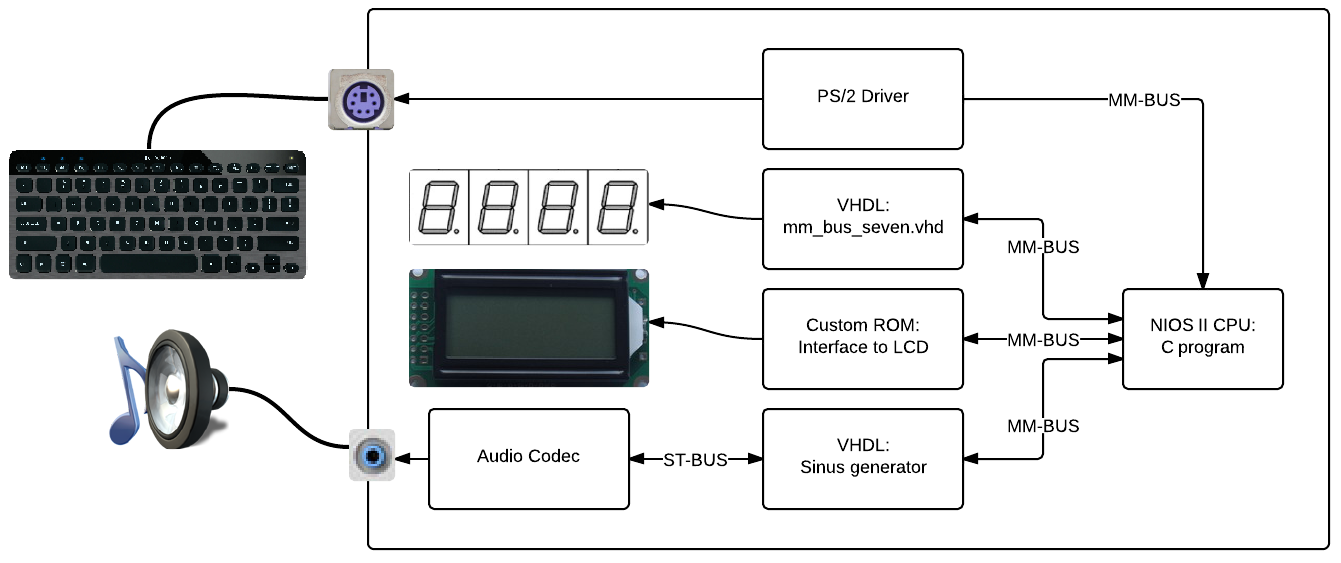
\includegraphics[scale=0.4]{Opstilling.png}
\caption{Opstilling}
\label{fig:opstilling}
\end{figure}


\end{document} 